\section{Policy responses}
\label{sec:policy}

If the shock modelled above is structural rather than cyclical---a permanent reallocation of labour demand rather than a downturn that unwinds---then the question facing the state is not whether the existing tax-benefit system cushions the blow (Section~\ref{sec:results} shows that it does, absorbing roughly half of the market-income loss) but whether it cushions it well, and at what fiscal cost the residual hardship could be bought down. This section evaluates three stylised policy responses inside the shocked world. Each reform is simulated on top of the central scenario (7 per cent displacement, seed 0, 2026), so the estimand throughout is the difference between the shocked-plus-reform and shocked simulations: what the reform adds, given that the shock has happened. I make no claim about the merits of these instruments in the absence of the shock, and the reforms apply for 2026 only---they are circuit breakers, not permanent settlements.

\subsection{Three stylised reforms}
\label{sec:policy-reforms}

The first reform (R1) is a wage-insurance scheme in the spirit of trade-adjustment proposals: displaced workers receive 50 per cent of their lost earnings, capped at \pounds 15{,}000 per year. I implement it as a post-simulation transfer that is non-taxable and disregarded by means tests, so its gross cost equals its net cost; this brackets the generous end of plausible implementations. The second (R2) is a demand-side circuit breaker within the existing architecture: a 20 per cent increase in the Universal Credit standard allowance, implemented as a parameter reform inside PolicyEngine so that all interactions with tapers, caps and passported entitlements are captured. The third (R3) suspends the benefit cap and cuts the UC earnings taper from 55 to 45 per cent, targeting the households for whom the existing system's own restraints bind hardest. R2 and R3 costs are net of clawback through the rest of the system.

\begin{table}[htbp]
\centering
\caption{Policy reforms on top of the central shock, 2026 (exposure-proportional incidence, seed 0)}
\label{tab:policy}
\small
\begin{tabular}{lcccccc}
\toprule
Reform & Cost & \multicolumn{2}{c}{$\Delta$ poverty (pp)} & $\Delta$ Gini & \multicolumn{2}{c}{\pounds bn per pp averted} \\
 & (\pounds bn) & BHC & AHC & (pp) & BHC & AHC \\
\midrule
R1 Wage insurance & 21.2 & $-1.53$ & $-1.65$ & $-0.97$ & 13.8 & 12.8 \\
R2 UC allowance $+20\%$ & 5.8 & $-0.64$ & $-0.56$ & $-0.31$ & 9.1 & 10.4 \\
R3 Cap suspension $+$ taper cut & 4.7 & $-0.46$ & $-0.45$ & $-0.23$ & 10.2 & 10.3 \\
\bottomrule
\end{tabular}

\medskip
\parbox{0.92\textwidth}{\footnotesize\emph{Note:} All effects are shocked-plus-reform minus shocked, fixed seed-0 draw, reforms in force for 2026 only. R1: 50 per cent of lost earnings, \pounds 15{,}000 cap, paid to 1.61 million displaced workers (mean transfer \pounds 13{,}173), modelled as non-taxable and means-test-disregarded so gross cost equals net cost. R2 and R3 are PolicyEngine parameter reforms; costs are net of clawback. R3 combines benefit-cap suspension with a UC taper cut from 55 to 45 per cent. Poverty lines are held at their shocked-world values.}
\end{table}

Table~\ref{tab:policy} reports the results and Figure~\ref{fig:policy} plots the decile pattern of the gains. The headline comparison is one of cost-effectiveness. The UC uplift averts a percentage point of after-housing-costs poverty for \pounds 10.4 billion, and the cap-and-taper package for \pounds 10.3 billion, against \pounds 12.8 billion for wage insurance. The reason is mechanical but instructive: wage insurance is earnings-proportional, and because the exposure-proportional shock displaces workers who are disproportionately in the upper half of the distribution, roughly 51 per cent of the R1 benefit is experienced in baseline deciles 8--10 (measured as a person-weighted household-gain share rather than a strict pound share). The UC-side instruments, by contrast, concentrate 71 per cent (R2) and 67 per cent (R3) of their benefit in deciles 1--5. Wage insurance does buy roughly three times more total poverty reduction than either UC reform---it is by far the largest intervention---but at roughly four times the cost, and with the weakest targeting per pound.

\begin{figure}[htbp]
\centering
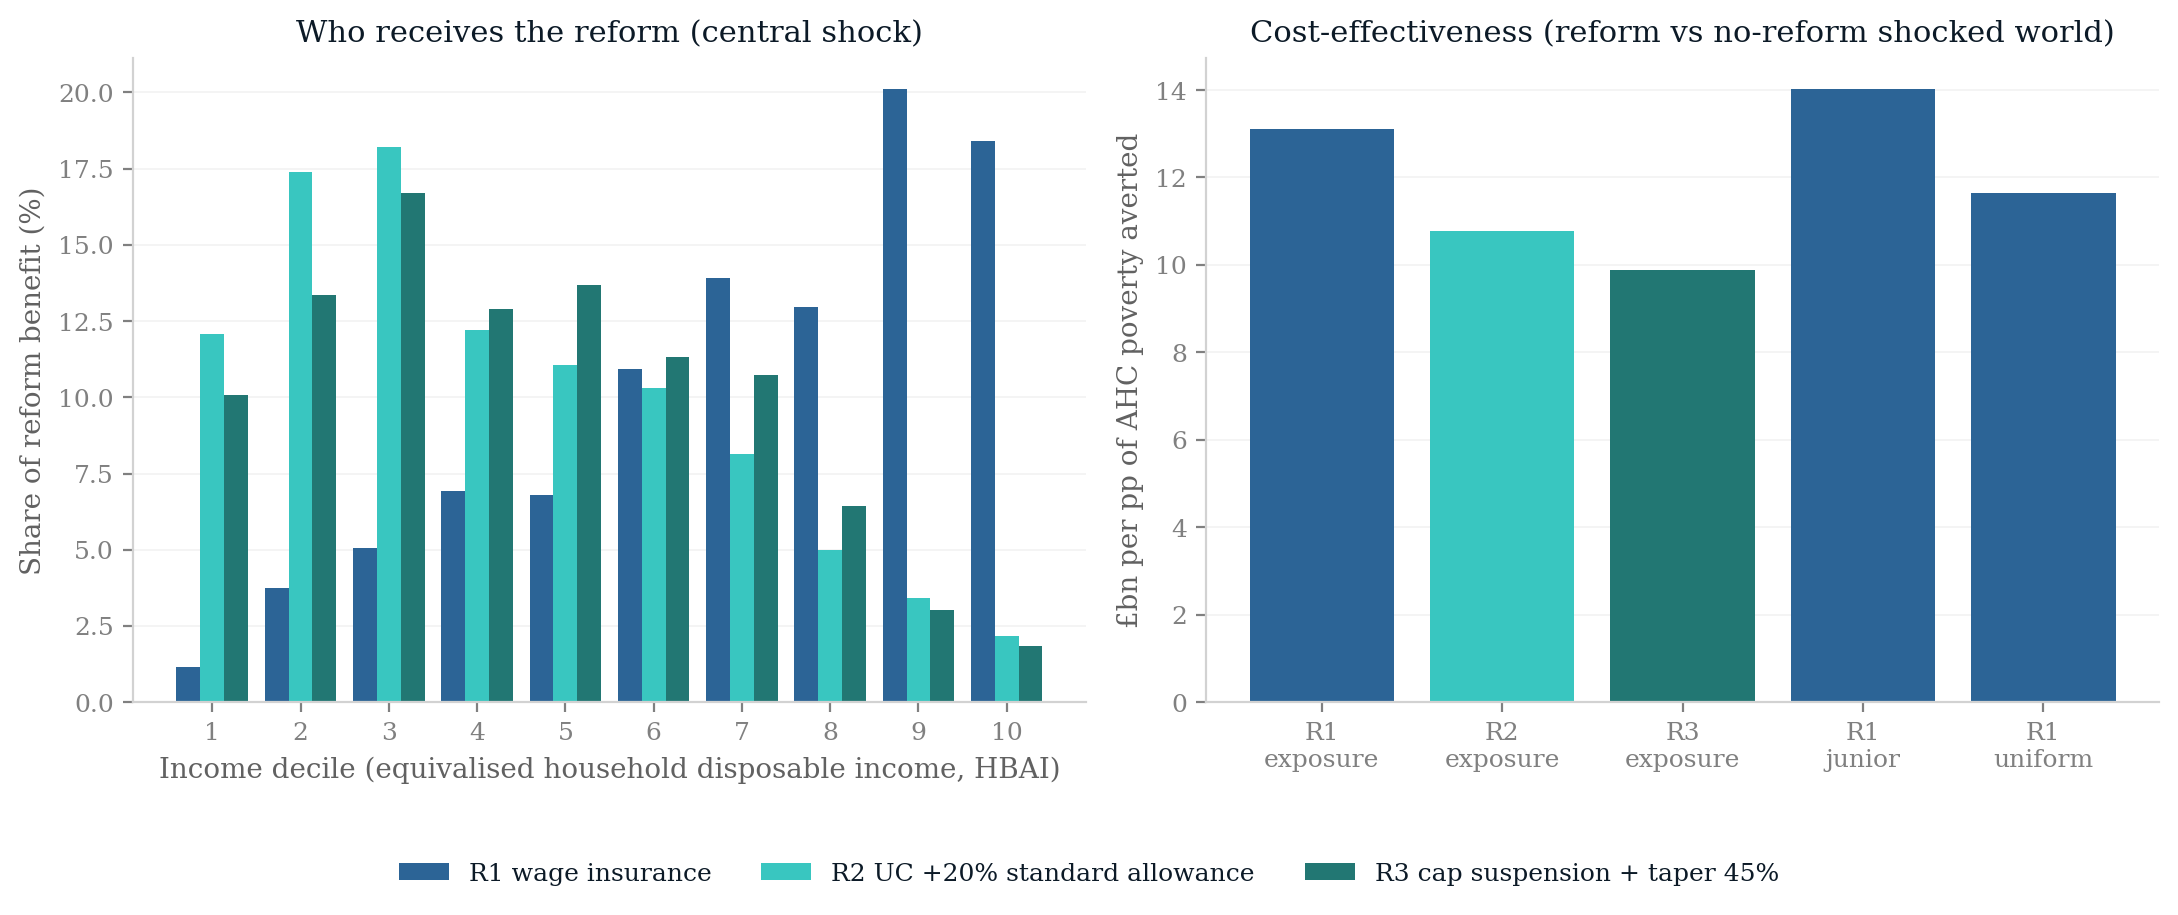
\includegraphics[width=.95\textwidth]{../results/policy/policy_reforms.png}
\caption{The three policy reforms on top of the central shock: fiscal cost, poverty and Gini effects, and the decile distribution of household gains. All panels show shocked-plus-reform minus shocked, seed 0, 2026.}
\label{fig:policy}
\end{figure}

The reform comparisons are far less sensitive to the displacement draw than the shock aggregates: over 20 Monte Carlo draws the wage-insurance cost varies by only $\pm$\pounds 0.2 billion (\pounds 21.4 $\pm$ 0.2 billion under exposure incidence, averting $1.44 \pm 0.10$ BHC points), and the UC-side instruments by less (R2: \pounds 5.69 $\pm$ 0.03 billion, $-0.54 \pm 0.02$ points; R3: \pounds 4.57 $\pm$ 0.06 billion, $-0.47 \pm 0.03$ points), so the cost-effectiveness ranking survives the draw noise comfortably. It also survives---indeed strengthens under---the six-month duration variant of Section~\ref{sec:results-aggregates}: with displaced workers recovering half a year's earnings, a duration-consistent wage insurance costs \pounds 33 $\pm$ 6 billion per BHC poverty point averted against \pounds 11.0 $\pm$ 0.6 billion for the UC uplift, because shortening the earnings loss shrinks the poverty problem faster than it shrinks the earnings-proportional transfer. Because Section~\ref{sec:results-incidence} established that incidence is the paper's central uncertainty, I re-run the wage-insurance reform under the junior-concentrated and uniform incidence families. The cost-effectiveness ranking is robust: R1 costs \pounds 14.3 billion per AHC point under junior incidence and \pounds 11.8 billion under uniform incidence, so even in its most favourable incidence world wage insurance only just reaches the \pounds 10.3--10.4 billion achieved by the UC-side instruments under the central family. The gross cost of R1 is nearly invariant across families (\pounds 20.3--21.4 billion), as it must be when the aggregate displaced wage bill is held approximately fixed; what varies is how much of that spending lands near the poverty line.

None of this settles the choice of instrument. Wage insurance addresses a different objective---consumption smoothing and earnings-loss compensation for the displaced themselves, most of whom are not poor---and a government persuaded by that objective would not be deterred by an unfavourable poverty-targeting ratio. What the exercise shows is narrower: if the criterion is poverty averted per pound in the shocked world, the existing means-tested architecture, temporarily made more generous, dominates a new earnings-linked scheme, precisely because the shock modelled here falls disproportionately on households that means tests are designed to exclude.

\subsection{The tax-composition channel}
\label{sec:policy-tax}

The reforms above spend money into a fiscal position that the shock has already damaged, and the size of that damage depends on a question the microsimulation cannot answer by itself: where does the displaced wage bill go? The OBR's recent analysis of AI-related fiscal risks \citep{obr2026} emphasises that labour displacement erodes the income-tax and National Insurance base even if aggregate output is unchanged, with the fiscal outcome hinging on how much of the lost labour income reappears as taxable profit. I price this channel on top of the microsimulation with a simple accounting exercise. Let $\phi$ denote the share of the displaced wage bill that reappears as corporate profits taxed at the 25 per cent main rate. In the central scenario the displaced wage bill is \pounds 77.9 billion and the effective income-tax-plus-NICs rate on displaced workers' earnings is 25.0 per cent, so the labour tax forgone is \pounds 19.5 billion---and because that effective labour rate almost exactly equals the corporation-tax main rate, the shortfall is very nearly $(1-\phi) \times 0.25 \times$ the displaced wage bill. At $\phi=0$ the net revenue shortfall is the microsimulation's \pounds 21.5 billion; at $\phi=0.5$ it falls to \pounds 11.8 billion; and at $\phi=1$ the labour-to-capital channel is almost exactly self-financing (a \pounds 0.03 billion surplus relative to full labour taxation), leaving only a residual \pounds 2.1 billion net cost, chiefly shock-induced benefit spending together with smaller non-labour-tax revenue changes. Figure~\ref{fig:phi} traces the full grid over displacement rates and $\phi$.

\begin{figure}[htbp]
\centering
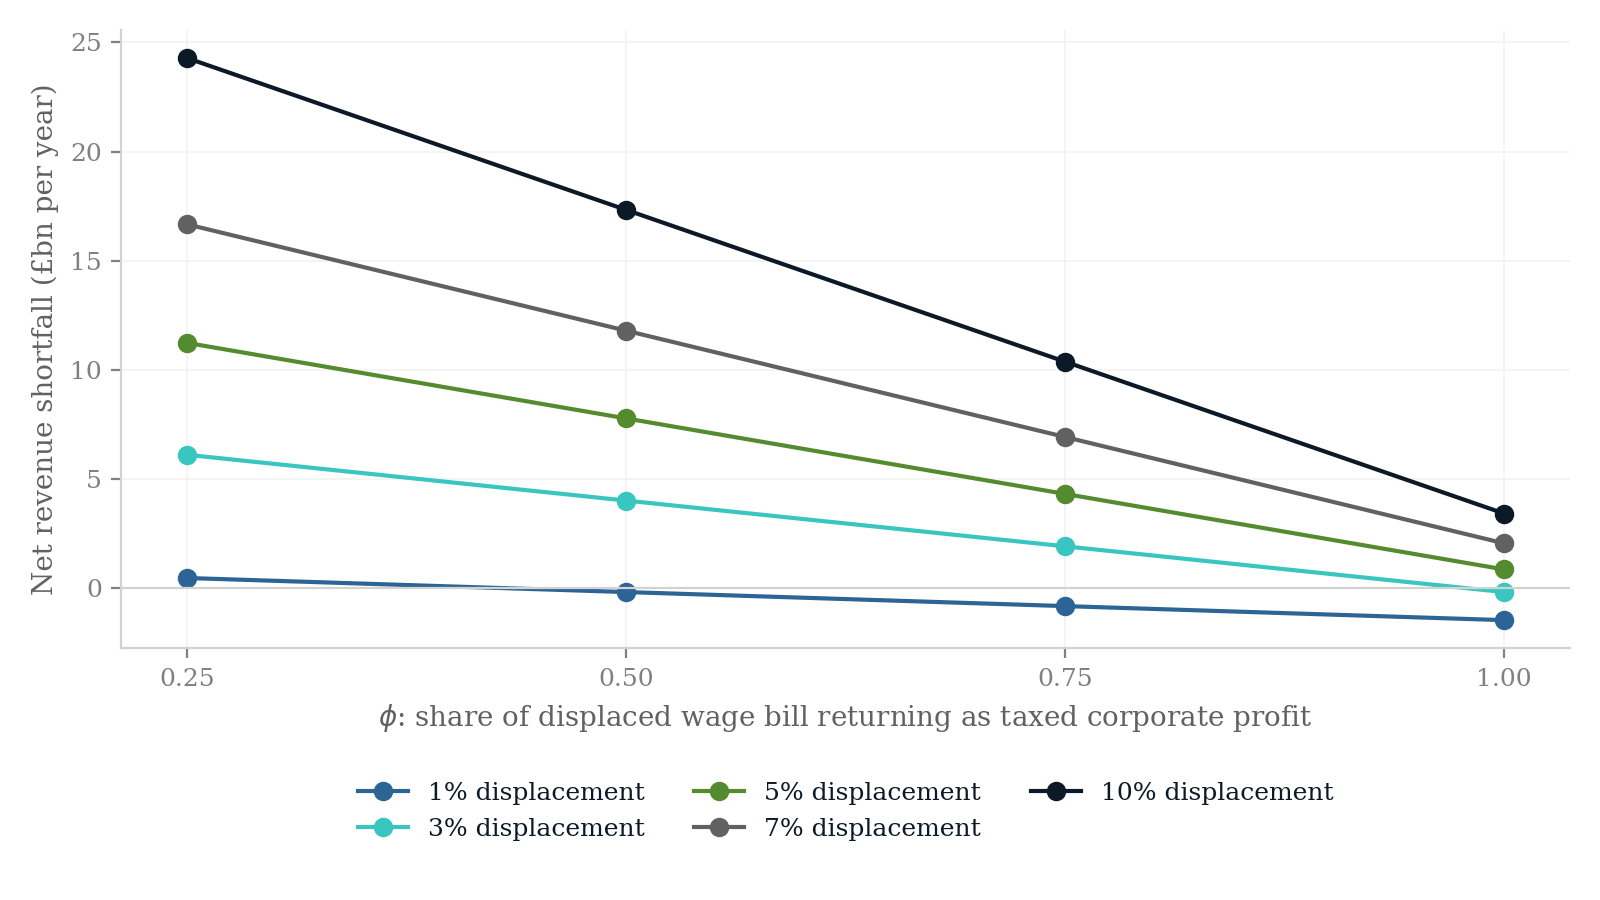
\includegraphics[width=.85\textwidth]{../results/tax_composition/revenue_shortfall_phi.png}
\caption{Net revenue change by displacement rate and $\phi$, the share of the displaced wage bill reappearing as corporate profits taxed at 25 per cent. The $\phi=0$ line is the microsimulation's net revenue change; higher $\phi$ adds recouped corporation tax outside the simulation.}
\label{fig:phi}
\end{figure}

Revenue neutrality, however, is not distributional neutrality. To see who receives the recomposed income, I simulate a dividend-recycling case at $\phi=0.5$ with a payout ratio of 0.5 (a parameter, not an estimate): \pounds 19.5 billion of post-CT profits are distributed pro rata to existing FRS dividend holders, with the dividend tax on those distributions captured inside the simulation. The result is stark. The Gini rises by a further 0.62 percentage points relative to the shocked world without recycling, and poverty---before or after housing costs---moves by exactly zero: the recycled dividends reach no household near the poverty line. The decile pattern of the gains is lumpy because FRS dividend records are sparse, but the message is not: deciles 1--4 receive exactly nothing. Even in the most fiscally benign reading of the shock, in which the Exchequer recovers essentially all of the lost labour tax through the corporate channel, the compositional shift from wages to capital income leaves the bottom of the distribution no better off and the overall distribution more unequal---which is precisely the configuration in which the transfer-side instruments of Section~\ref{sec:policy-reforms} would be needed most.

Two caveats bound this exercise. It is static accounting layered on top of the microsimulation: the incidence of corporation tax is not modelled, the corporation-tax base is assumed equal to accounting profit (no allowances, losses or profit shifting), and the effective labour rate is a pro-rata attribution of income tax and NICs to employment income that ignores the schedule ordering of savings and dividend bands. And $\phi$ itself is the free parameter the whole channel turns on; I present a grid rather than a point estimate because nothing in my framework pins it down.
